\documentclass[12pt]{article}

\usepackage{sbc-template}

\usepackage[brazil]{babel}
\usepackage[utf8]{inputenc}

\usepackage{url}
\usepackage{graphicx}
\usepackage{float}

\graphicspath{{\main/imagens/}{imagens/}}

\sloppy

\title{
    Desenvolvimento de documentação e implementação de sistema de informação para
    contribuir na formação do perfil de analista de sistemas
}

\author{Vinícius B. Bruscagini\inst{1}, Carlos R. S. Júnior\inst{1}}

\address{
    Instituto Federal de Educação, Ciência e Tecnologia do Estado de São Paulo\\
    Campus Hortolândia (IFSP-HTO)
    \email{vinicius.bruscagini@aluno.ifsp.edu.br, carlos.rsantos@ifsp.edu.br}
}

\begin{document}

\maketitle

\begin{abstract}
  Given the challenges for IT Universities to adapt their curriculum in regarding to new tecnologies
  due to the fast-growing-market, this paper has a main objective to make avaliable a technical
  documentation of a developed software with consolidated technologies in the market to collaborate with the
  formation of IT Students.
\end{abstract}

\begin{resumo}
    Dado o desafio das instituições de ensino da área de tecnologia em adequar os conteúdos abordados
    às novas tecnologias devido a rápida evolução do mercado, este trabalho tem como principal objetivo
    disponibilizar uma documentação técnica de um software desenvolvido com tecnologias consolidadas no mercado
    afim de colaborar na formacão de alunos do curso de Análise e Desenvolvimento de Sistemas.
\end{resumo}

\section{Introdução}

A área de TI (Tecnologia da Informação), é uma área que evoluiu muito nas últimas
décadas~\cite{Pacheco10} e continua evoluindo rapidamente. Novas tecnologias e ferramentas
surgem em rítmo acelerado e muitas delas ganham popularidade, demandando assim, novas
habilidades para os profissionais de TI\@. Com essa evolução, surge um desafio para as
instituições de ensino atualizarem seus conteúdos, o principal fator para esse problema
é a burocracia para a atualização das ementas de disciplinas. Isso faz com que
muitos desses busquem cursos ou certificações para aprimorar seus conhecimentos~\cite{macedo09}.
Além disso, de acordo com uma pesquisa realizada por~\cite{wei08} os alunos de cursos de como Engenharia de \textit{Software}
se preocupam em possuir um aprendizado voltado para prática e em ter convivência com conceitos
e métodos importantes para o mercado de trabalho.

Baseando-se nessas questões, a produção desse trabalho tem a proposta de desenvolver
um sistema com tecnologias e ferramentas populares que possuem demanda por profissionais,
com o objetivo principal de construir uma documentação
que abrange os aspectos desse sistema e que explique com clareza como o software
funciona, quais tecnologias foram usadas e como se deu o seu desenvolvimento. Assim ajudando estudantes a
entenderem alguns conceitos de desenvolvimento de software e como se dão suas aplicações na prática.

Neste trabalho, então, a solução desenvolvida possui o nome de `Foryum' e esse sistema foi desenvolvido
com tecnologias escolhidas baseadas em pesquisas que são detalhadas na seção~\ref{Desenvolvimento},
foram elas \textit{.NET} e \textit{Vue.js}. Além da solução técnica, foi criada a documentação dessa solução, que é
importante para o entendimento do código fonte. Esses materiais estão disponíveis na plataforma \textit{GitHub} nos
\textit{links} mostrados na seção~\ref{Resultados} de Resultados. Com o desenvolvimento de um \textit{software}
e de sua documentação, espera-se que a disponibilização desses materiais
possa colaborar com estudantes dos cursos de Análise e Desenvolvimento de Sistemas pois esse material mostra como funciona um ambiente
real de \textit{software}.

Esse artigo possui a seguinte organização: a Seção~\ref{FundamentacaoTeorica} nomeada Fundamentação Teórica,
evidencia em subseções os conceitos empregados durante o desenvolvimento deste trabalho. Na sequência,
a Seção~\ref{Metodologia} nomeada Metodologia, descreve o processo realizado para esse desenvolvimento.
A Seção~\ref{Desenvolvimento}, Desenvolvimento do Trabalho, mostra as etapas de desenvolvimento para chegar ao objetivo do trabalho, divididos em subseções.
A Seção~\ref{Resultados} de Resultados, mostra o que foi implementado e documentado de acordo com o objetivo do trabalho.
Por último a Seção~\ref{Conclusao}, Conclusão, resume todo o artigo e mostra possíveis trabalhos futuros.

\section{Fundamentação Teórica}\label{FundamentacaoTeorica}

Nessa seção são apresentados conceitos relacionados ao desenvolvimento de \textit{software} e gerenciamento
de projetos. Esses conceitos foram empregados para realizar o desenvolvimento do \textit{software} conforme descrito na seção anterior.

\subsection{Framework}

De acordo com~\cite{host12} um
\textit{framework} é como um template que conta com diversas funcionalidades que possui o objetivo principal de
resolver problemas recorrentes no desenvolvimento e acelerar esse processo.

\subsection{WebService}\label{WebService}

Um \textit{WebService} é um serviço que é oferecido e é por onde aplicações se comunicam com o servidor.
WebServices fazem parte da arquitetura orientada a serviços (SOA).

Um tipo de \textit{WebService} muito utilizado é o REST, que significa
\emph{Representational State Transfer} que funciona servindo requisições de clientes
para certos serviços. Por exemplo, suponha que um \textit{WebService} REST tenha uma \textit{URL} que fornece
informações de funcionários:

\begin{verbatim}
  GET http://meuwebservice/funcionarios
\end{verbatim}

\textit{GET} é o método HTTP usado para requisitar as informações que queremos, então se enviarmos uma requisição
para a URL com o método esperado, o \textit{WebService} irá responder a requisição com dados em formato \textit{JSON}
com as informações que queremos, um exemplo de uma resposta \textit{JSON} é mostrada na Figura~\ref{fig:json}.

\begin{figure}[h]
    \centering
    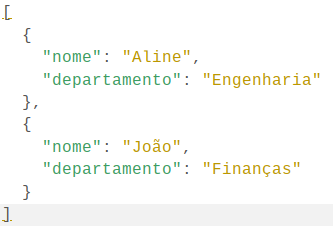
\includegraphics[width=0.5\textwidth]{code/json.png}
    \caption{Exemplo de JSON como resposta}\label{fig:json}
\end{figure}

Um \textit{WebService} REST pode ter vários URLs, também chamadas de \textit{endpoints}, além de obter informações, podemos realizar
diferentes operações em diferentes \textit{endpoints}, como inserir um objeto no sistema, por exemplo.

\subsection{Qualidade de Software}

A definição de qualidade no contexto da computação nem sempre é um consenso,
existem diferentes terminologias, as quais podem causar problemas para pessoas que não
possuem conhecimento sobre~\cite{Duarte03}.

Um \textit{software} pode ser considerado de qualidade quando ele atende a todas as necessidades, explicitas
e implícitas para qual ele foi feito~\cite{Duarte03}. Além disso, um \textit{software} é composto por um código fonte.
Existem padrões que devem ser seguidos para um código possuir qualidade.
Devemos pontuar que para isso, ele deve funcionar, e principalmente, ser legível.

De acordo com~\cite{Levy04}: ``Muitos programadores iniciantes acham que um bom código é aquele que é correto, ou seja, faz o que tem
que fazer''.

Um código, para funcionar deve possuir ao menos duas características, ele deve ser \textbf{Correto} e \textbf{Eficiente},
esses pontos são o que fazem um código funcionar. Porém isso não é o suficiente para ser considerado
um código de qualidade. No mundo real, códigos são criados, alterados e revistos, geralmente por diferentes pessoas,
por isso existem duas propriedades adicionais que um código deve possuir, ele deve ser \textbf{Elegante} e \textbf{Testável}
como descritos por~\cite{Levy04}.

Um código elegante e testável dá qualidade ao nosso código pois isso facilita, e muito, sua manutenção.

\subsection{Controle de Versão}

Controle de versão é a prática de rastrear e gerenciar mudanças no código do \textit{software}~\cite{attlasianGit}.
Essas ferramentas gerenciam o código fonte de projetos ao longo do tempo, e possuem informações detalhadas
de todas as modificações que foram realizadas em todos os arquivos do código fonte.
Alguns dos benefícios que essas ferramentas proporcionam são rastreabilidade (quem fez o quê),
ajudam na resolução de conflitos e aceleram o desenvolvimento. A ferramenta mais famosa para controle de
versão atualmente é o \textit{Git}.

\subsubsection{Git}

O \textit{Git} é a ferramenta mais usada para controle de versão. De acordo com seu website, ele
funciona com o conceito de \textit{commits} e \textit{branches}, em que um \textit{commit}
é uma alteração realizada no código, e uma \textit{branch} é uma ramificação do código, elas são
exemplificadas na Figura~\ref{fig:git-branches} que mostra três \textit{branches} de um repositório,
uma chamada \textit{master}, outra de \textit{Feature 1} e uma outra chamada \textit{Feature 2}.

\begin{figure}[h]
  \centering
  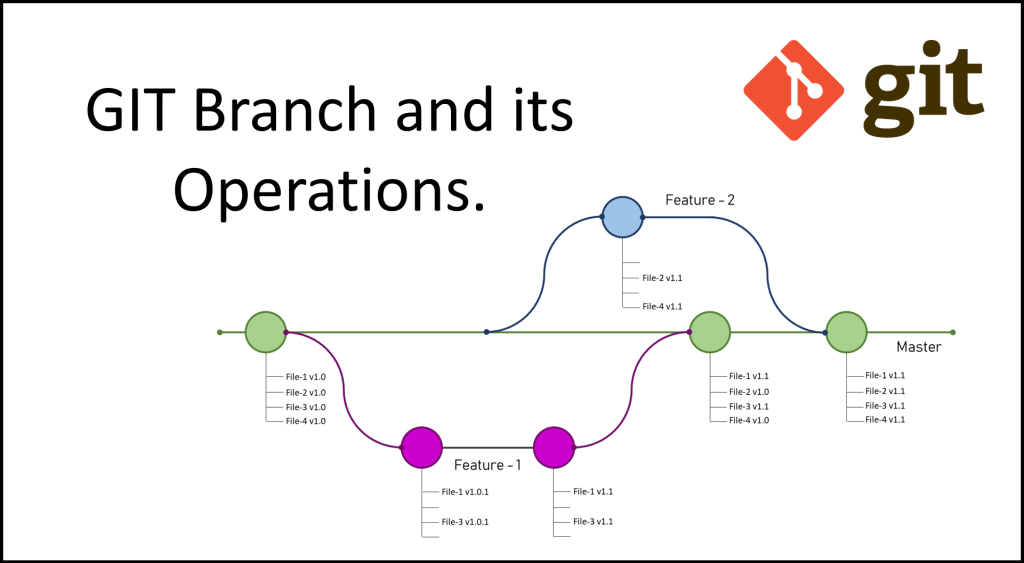
\includegraphics[width=1\textwidth]{git/git-branches.png}
  \caption{Exemplos de branches em um repositório Git}\label{fig:git-branches}
\end{figure}

Durante o desenvolvimento de um \textit{software}, essas ramificações acontecem frequentemente. Nesse exemplo,
há duas ramificações que foram criadas para desenvolver uma funcionalidade no \textit{software}, também chamado de \textit{feature},
ou seja, a partir de uma \textit{branch} principal \textit{Master}, foram criadas duas \textit{branches} onde o desenvolvimento
de uma funcionalidade foi feita, e ao final desse desenvolvimento, o código feito nessa \textit{branch} foi
unido junto com a \textit{branch} principal.

Com o \textit{software} instalado em um computador podemos usar o comando \verb|git| para realizarmos operações.
Um típico fluxo de um desenvolvimento usando \textit{Git} é mostrado na Figura~\ref{fig:git-lifecycle}.

O \textit{Git} funciona em repositórios, que é uma pasta onde estão os arquivos de código de um sistema,
a partir desse repositório, modificações são feitas no código, as quais são adicionadas em um \textit{commit}
e esse \textit{commit} é enviado para um repositório remoto, onde outras pessoas da equipe podem obter as modificações feitas.

\begin{figure}[h]
  \centering
  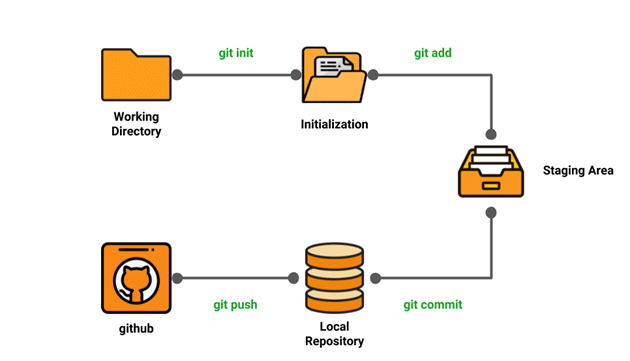
\includegraphics[width=.8\textwidth]{git/git-lifecycle.png}
  \caption{Típico ciclo de desenvolvimento com Git}\label{fig:git-lifecycle}
\end{figure}

\subsection{Documentação de Software}

De acordo com~\cite{Forward02softwaredocumentation}, a documentação de um \textit{software} é qualquer
artefato que possui como finalidade informar sobre ele, em qualquer um de seus aspectos.

~\cite{Coelho_2009} nos mostra dois tipos de documentações, são esses tipos:

\begin{itemize}
	\item Documentação Técnica;
	\item Documentação de Uso.
\end{itemize}

As documentações técnicas de um sistema é toda aquela documentação voltada ao desenvolvedor, esse material
informa como o sistema funciona internamente, sua arquitetura, tecnologias usadas e outros detalhes de implementação.

As documentações de uso são documentos que são focados nos usuários finais do sistema e as vezes também em administratores.
Essas documentações geralmente mostram como usar o sistema.

Ambos os tipos de documentações são muito importantes no processo de desenvolvimento e entrega de \textit{softwares}.
A falta ou baixo nível de qualidade de documentações atrapalham na compreensão do sistema e podem apresentar
riscos para sua manutenção~\cite{deinvestigaccao}.

\subsection{Metodologias Ágeis}

As metodologias ágeis surgiram na década de 80 para melhorar a área de desenvolvimento de software,
que era algo muito rigoroso naquela época, muitos projetos possuiam problemas e as metodologias ágeis foram então
criadas para tentar solucioná-los~\cite{Santos05}.

\subsubsection{Kanban}

O \textit{Kanban} funciona com quadros, chamados de quadro \textit{Kanban}, onde um quadro é constituido por colunas e
em cada coluna pode-se definir tarefas.

Em um quadro Kanban podemos agrupar tarefas, definir datas e responsáveis para essas tarefas, entre vários outros
detalhes, o que facilita a organização e visão do trabalho a ser realizado em um projeto.

Existem várias ferramentas que oferecem um quadro \textit{Kanban} para o gerenciamento de tarefas.
Uma delas é o \emph{GitHub Projects}, que é usada neste trabalho. A interface desse programa é mostrada na Figura~\ref{fig:github-board}.

\begin{figure}[h]
  \centering
  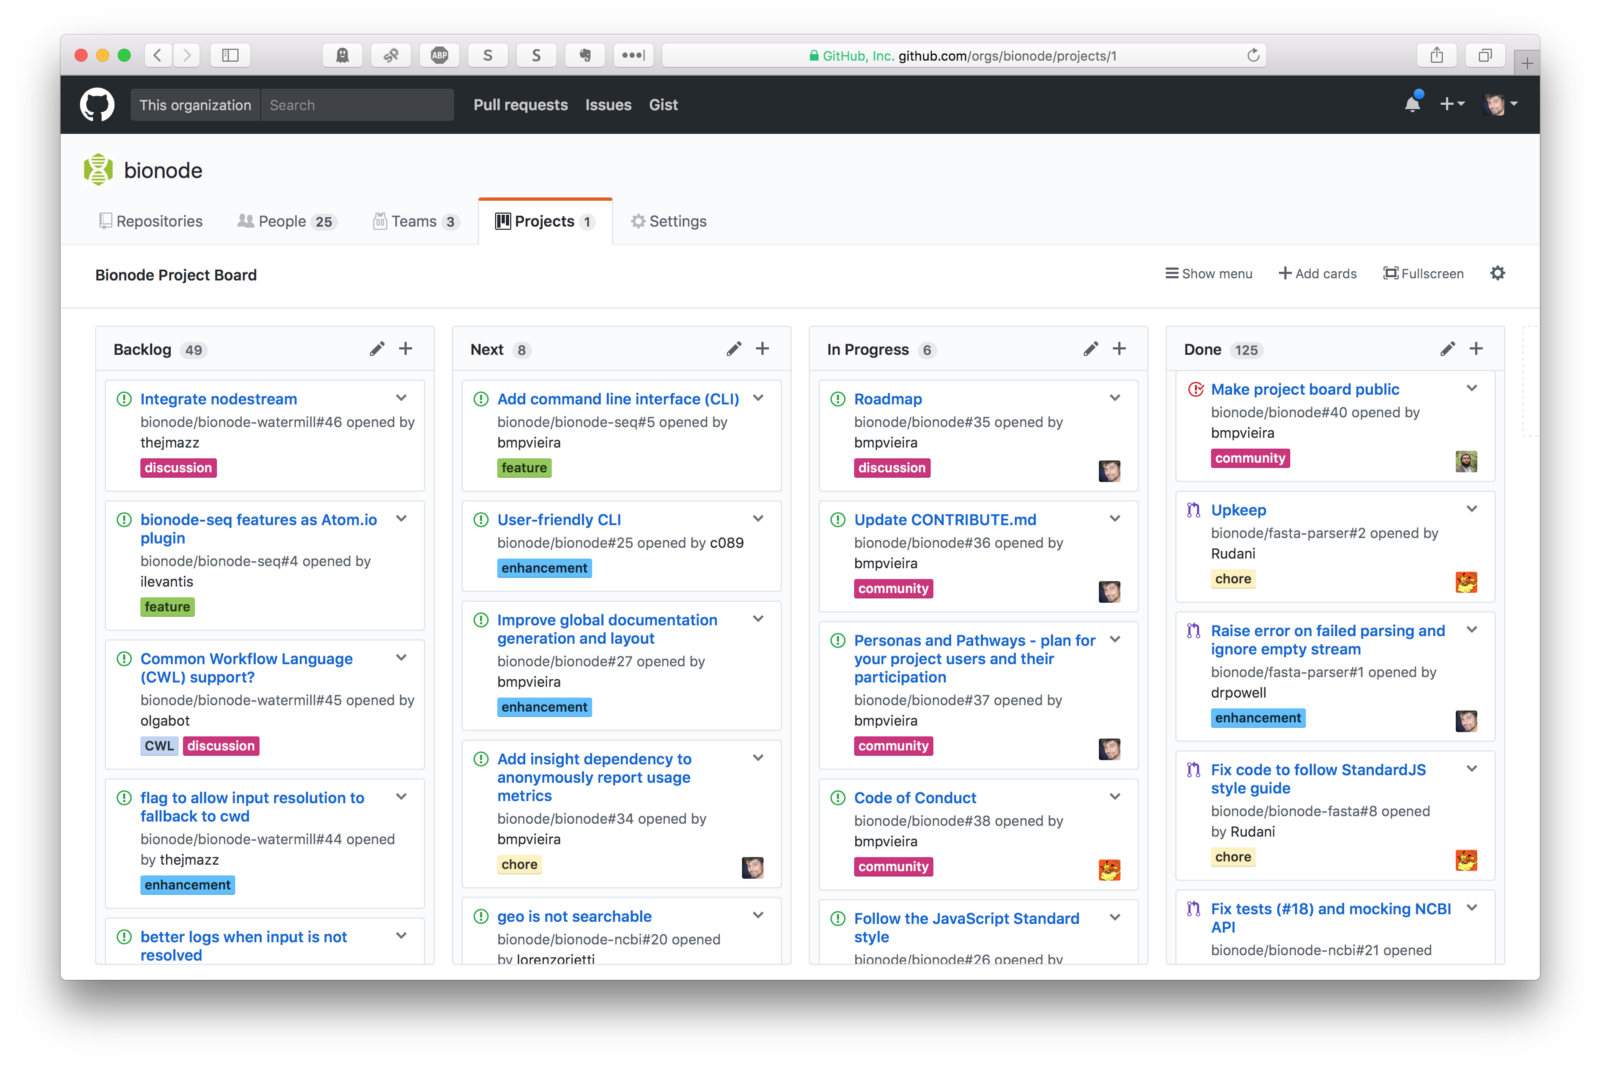
\includegraphics[width=1\textwidth]{github/github-board.png}
  \caption{Visão de um quadro \textit{Kanban} do \emph{GitHub Projects}}\label{fig:github-board}
\end{figure}


% TODO: Falar de um pouco de Testes unitários aqui

\section{Metodologia}\label{Metodologia}

Para início do desenvolvimento foi realizada a definição das tecnologias do sistema, para isso, foram feitas
pesquisas bibliográficas em \textit{WebSites} como \textit{GitHub} e \textit{Stackoverflow}. Estes \textit{WebSites}
são famosos na área de desenvolvimento, eles forneceram informações importantes sobre quais
são as tecnologias mais ativas, mais comentadas e outros dados que foram usados para a escolha das tecnologias
usadas no desenvolvimento do sistema.

Com as tecnologias definidas, o próximo passo foi a análise e documentação de requisitos do sistema,
e com esses requisitos, foram criados diagramas de classes e casos de uso.

Para o desenvolvimento, foram usados recursos oferecidos pela plataforma \textit{GitHub}, esses recursos são:

\begin{itemize}
  \item Repositório \textit{Git};
  \item Quadro \textit{Kanban} para o gerenciamento de tarefas;
  \item \textit{Wiki} onde foi criada a documentação técnica do sistema.
\end{itemize}

\section{Desenvolvimento do Trabalho}\label{Desenvolvimento}

Em Maio de 2021 foi realizada pelo site~\cite{stack11}, uma pesquisa com desenvolvedores de todo o mundo para
coletar dados geográficos, sociais e de uso de tecnologias de seus usuários. Esses dados nos permitem ter
informações importantes sobre o uso de tecnologias em geral. A pesquisa nos dá três conjuntos
de informações relevantes para usarmos no trabalho

\begin{itemize}
  \item Frameworks para Web mais utilizados;
  \item Frameworks gerais mais utilizados;
  \item Ferramentas para deploy e gerenciamento mais usadas;
  \item Banco de Dados mais utilizados.
\end{itemize}

Os resultados dessas categorias, entre desenvolvedores profissionais, são exibidos nas
Figuras~\ref{fig:web-frameworks},~\ref{fig:general-frameworks},~\ref{fig:tools} e~\ref{fig:databases}, respectivamente.

\begin{figure}[h]
  \centering
  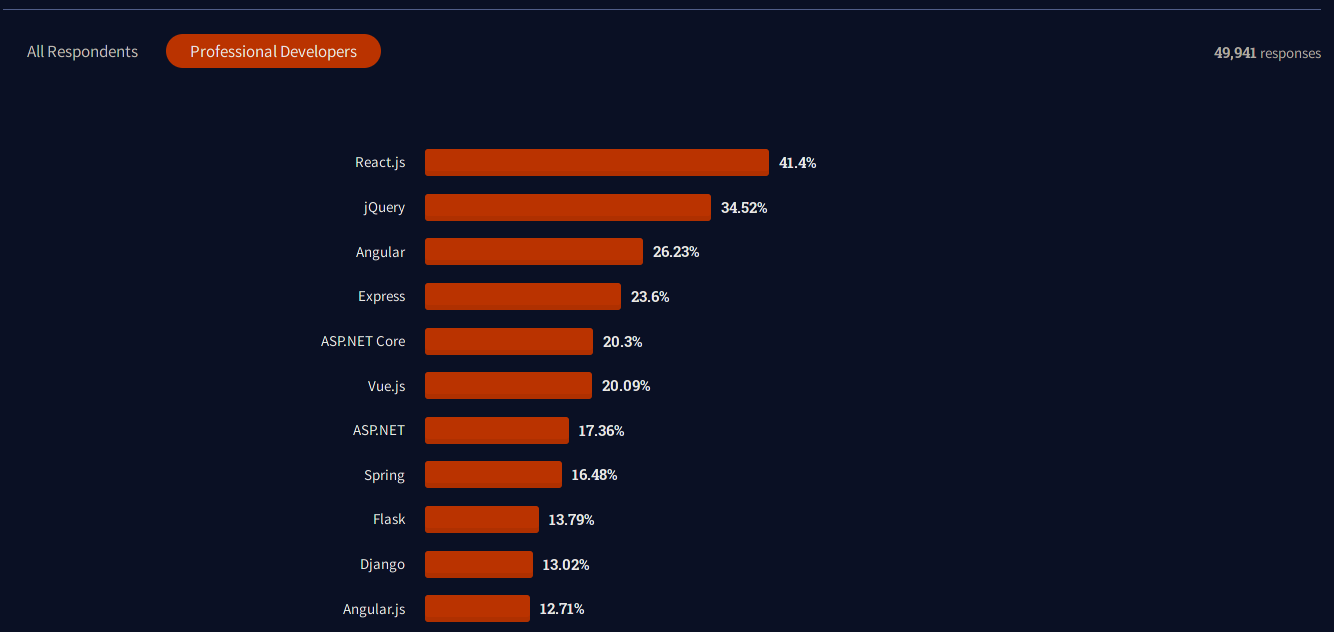
\includegraphics[width=0.9\textwidth]{stackoverflow/web_frameworks_usage.png}
  \caption{Gráfico mostrando os frameworks Web mais usados}\label{fig:web-frameworks}
\end{figure}

A Figura~\ref{fig:web-frameworks} mostra as tecnologias para desenvolvimento de aplicações Web mais populares entre desenvolvedores
profissionais que participaram da pesquisa, e mostra também a popularidade de \textit{frameworks JavaScript} para
desenvolvimento \textit{Web}, como \textit{React.js}, \textit{Angular}, \textit{Express} e \textit{Vue.js}.

\begin{figure}[h]
  \centering
  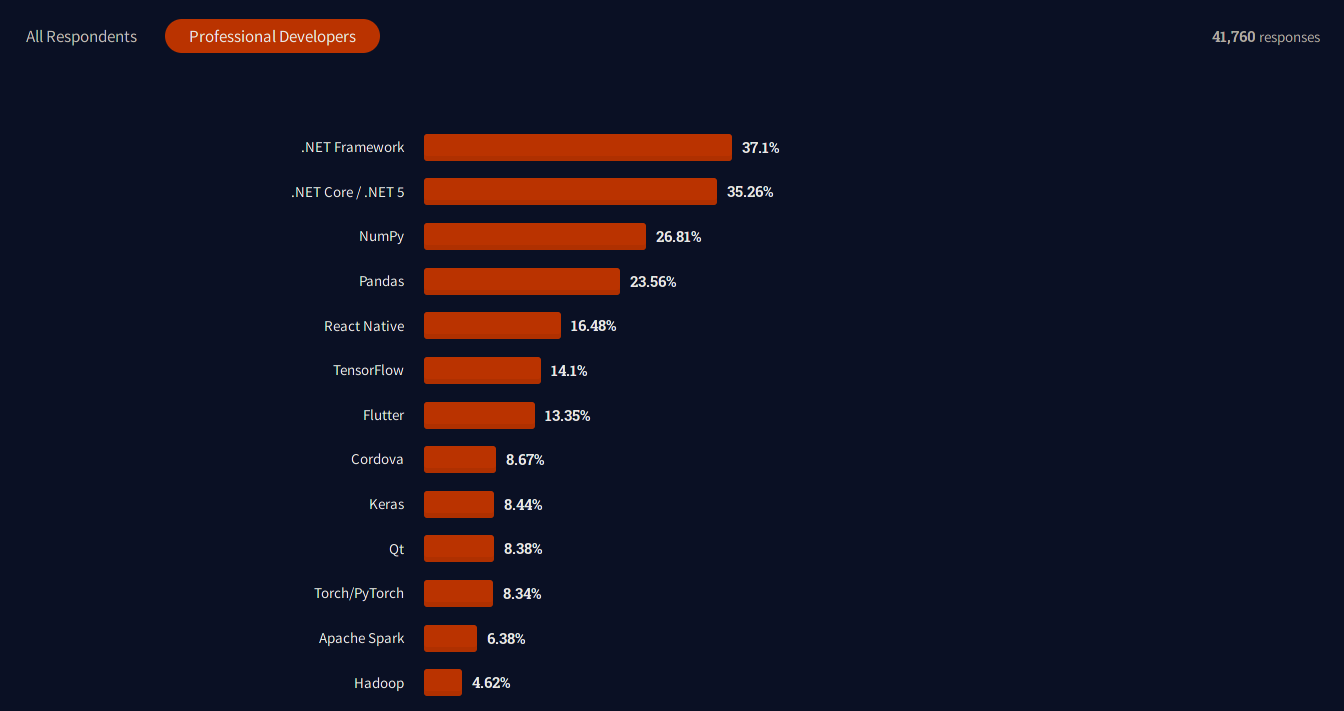
\includegraphics[width=0.9\textwidth]{stackoverflow/general_framework_usage.png}
  \caption{Gráfico mostrando os frameworks gerais mais usados}\label{fig:general-frameworks}
\end{figure}

A Figura~\ref{fig:general-frameworks} mostra o \textit{.NET Framework / .NET 5} como \textit{framework}
mais popular para o desenvolvimento geral de aplicações, outras tecnologias mostradas na pesquisa são específicas
para algum tipo de tarefa e não são genéricas para o desenvolvimento de aplicações, como \textit{NumPy} e \textit{Pandas}, por exemplo, que
são bibliotecas para análise de dados com a linguagem \textit{Python}~\cite{PandasPython}.

\begin{figure}[h]
  \centering
  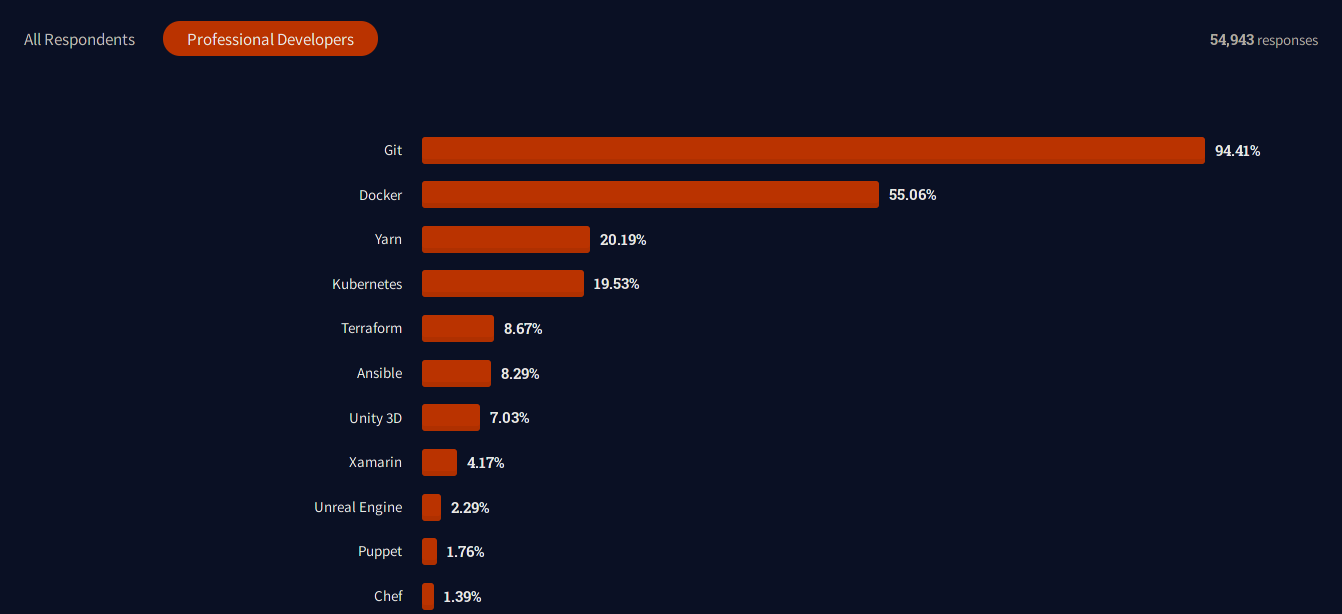
\includegraphics[width=0.9\textwidth]{stackoverflow/used_tools.png}
  \caption{Gráfico mostrando as ferramentas mais usadas}\label{fig:tools}
\end{figure}

A Figura~\ref{fig:tools} mostra as ferramentas mais populares presentes no ambiente de desenvolvimento dos desenvolvedores
que participaram da pesquisa. \textit{Git} e \textit{Docker} aparecem como ferramentas populares, sendo o \textit{Git} presente
na rotina de mais de 94\% dos participantes, isso mostra que o \textit{Git} é uma tecnologia bastante presente e que é
importante que o perfil de Analista de Sistema possua conhecimentos sobre essa ferramenta.

\begin{figure}[h]
  \centering
  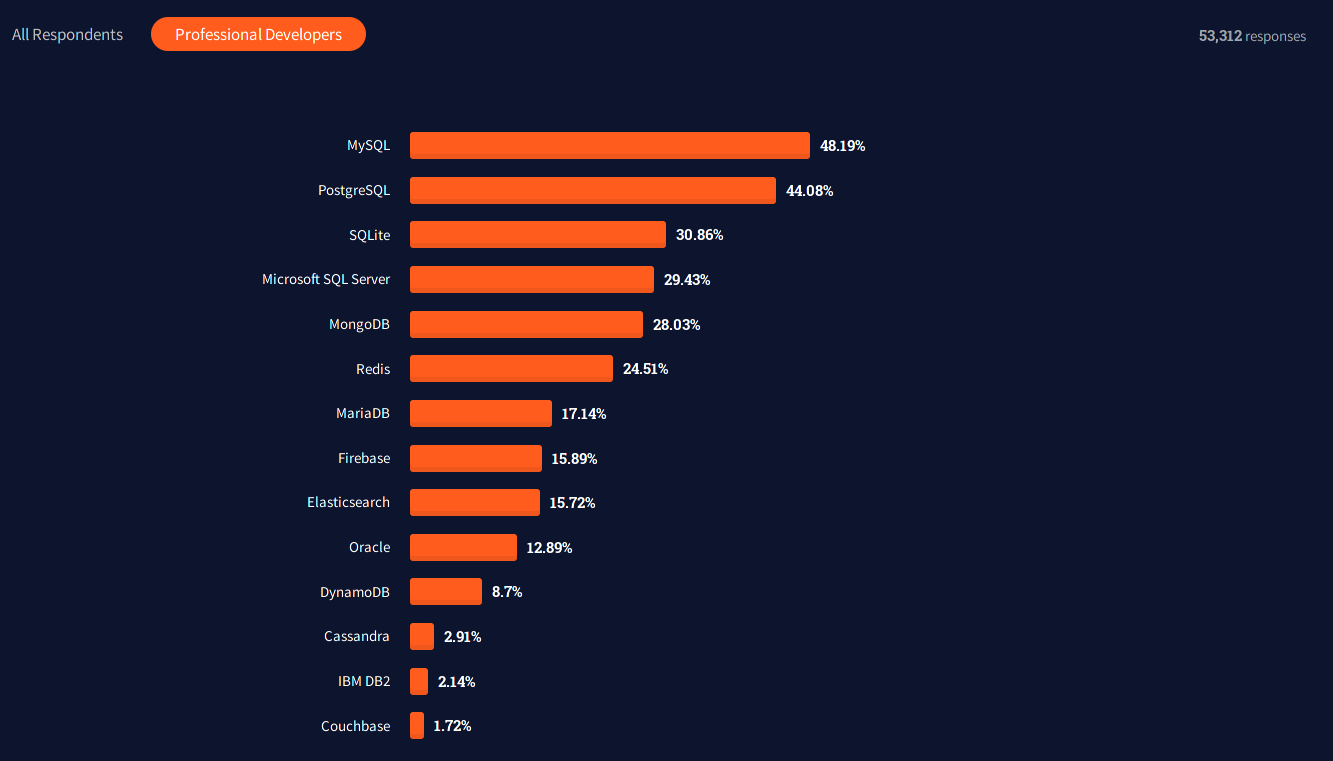
\includegraphics[width=0.9\textwidth]{stackoverflow/databases.png}
  \caption{Gráfico mostrando os SGBDs mais usados}\label{fig:databases}
\end{figure}

A Figura~\ref{fig:databases} mostra quais os SGBDs mais populares, sendo eles o \textit{MySQL} e o \textit{PostgreSQL}.

Baseando-se nos dados de popularidade indicados pela pesquisa do site \textit{Stack Overflow} e na experiência do autor em certas tecnologias e ferramentas,
foi optado o uso das tecnologias e arquitetura apresentadas na Seção~\ref{ArquiteturaTecnologias}.

\subsection{Arquitetura e Tecnologias}\label{ArquiteturaTecnologias}

A arquitetura escolhida para o sistema foi um \textit{WebService REST}, como mostrado na Seção~\ref{WebService}.
Além do \textit{WebService} foi decidido a criação de uma aplicação cliente que acesse o \textit{WebService}.

As tecnologias que foram usadas para a implementação dessas aplicações são apresentadas nas próximas seções.

\subsubsection{ASP.NET Core}

O \textit{ASP.NET Core} faz parte da família de tecnologias \textit{.NET} que são desenvolvidas pela \textit{Microsoft}.
Ele nos permite criar qualquer tipo de aplicação \textit{web}.

A Plataforma \textit{.NET} possui uma longa história, por grande parte dessa história, suas
tecnologias foram exclusivas para o sistema operacional \textit{Windows}. Em 2014 a \textit{Microsoft} recriou
essa plataforma do zero, hoje toda a plataforma é \textit{open-source} e funciona em qualquer
sistema operacional.

\subsubsection{\textit{Entity Framework Core}}

O \textit{Entity Framework Core} é um \textit{framework ORM} que é usado em conjunto com o \textit{.NET}
como explicitado por~\cite{ormHibernate}:

\begin{quote}
  ``Um \textit{framework ORM} provê uma metodologia e mecanismo
  para sistemas orientados a objetos manterem seus dados em um banco de dados de maneira
  segura, com controle de transações, e tudo isso expressado em código orientado a objeto''.
\end{quote}

De maneira prática, um \textit{ORM} permite manipularmos entidades em um banco de dados
sem precisarmos mexer com \textit{SQL}. Eles geralmente funcionam mapeando as classes
que criamos em nosso código, e com essas informações ele cria o banco de dados já com os relacionamentos
entre as tabelas e tudo mais o que definimos nas classes.

O \textit{Entity Framework} é o \textit{ORM} oficial do \textit{.NET}, possui amplo suporte e uso. Ele será
usado nesse projeto para facilitar a manipulação dos dados no banco de dados.

\subsubsection{Vue.js}

O \textit{Vue} é um \textit{framework} para desenvolvimento de aplicações \textit{web}, usando a linguagem \textit{JavaScript},
ele nos permite o desenvolvimento de aplicações reativas e possibilita o reuso
de código através de componentes. Abaixo um pequeno código \textit{HTML} de um arquivo vue

\begin{verbatim}
  <div>
    <p v-if="seen">Agora você me viu</p>
  </div>
\end{verbatim}

Esse trecho de código exibe o texto `Agora você me viu' caso a variável \verb|seen| seja verdadeira.

O \textit{Vue} nos dá a opção de usar a linguagem \textit{TypeScript} ao invês do \textit{JavaScript}, ele possui
várias bibliotecas que melhoram a legibilidade e arquitetura de um componente vue.
Abaixo um código de um componente \textit{Vue} usando \textit{TypeScript}

\begin{verbatim}
<template>
  <p>Texto</p>
</template>

<script lang="ts">
import Vue from "vue";
import Component from "vue-class-component";

@Component
export default class About extends Vue {

}
</script>
\end{verbatim}

O \textit{Vue} possui um ecosistema de bibliotecas adicionais para ajudar no desenvolvimento de aplicações.
Uma dessas bibliotecas é o \textit{Vuetify}, ele fornece para o desenvolvedor componentes para interface
como botões, \textit{cards}, campos de textos, etc.

\subsection{Definição de Requisitos}

Com o processo e as tecnologias definidas. O próximo passo foi de
definir o domínio do sistema a ser desenvolvido e seus requisitos.

Os requisitos do sistema foram baseados em um sistema já existente, essa aplicação
é o \textit{Reddit}, e o nome do sistema desenvolvido nesse trabalho é `Foryum'. O \textit{Reddit},
de acordo com seu website é: ``A casa de milhares de comunidades, conversas sem
limite e interação humana autentica.''

O \textit{Reddit} consiste de comunidades que tratam de determinado assunto, nessas comunidades, usuários
podem se inscrever e realizar postagens, as quais outros usuários dessa comunidade virão e podem
dar um voto positivo ou negativo para essa postagem.

Foram criados dois diagramas de casos de uso que representam as funcionalidades esperadas no sistema,
eles são apresentados nas Figuras~\ref{fig:welcome_diagram} e~\ref{fig:home_diagram}.

\begin{figure}
    \centering
    \begin{minipage}{0.45\textwidth}
        \centering
        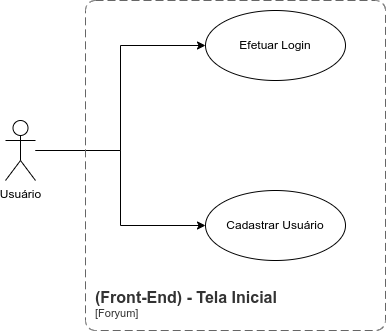
\includegraphics[width=0.9\textwidth]{diagrams/welcome_diagram.png}
        \caption{Diagrama de casos de uso da tela inicial}\label{fig:welcome_diagram}
    \end{minipage}\hfill
    \begin{minipage}{0.45\textwidth}
        \centering
        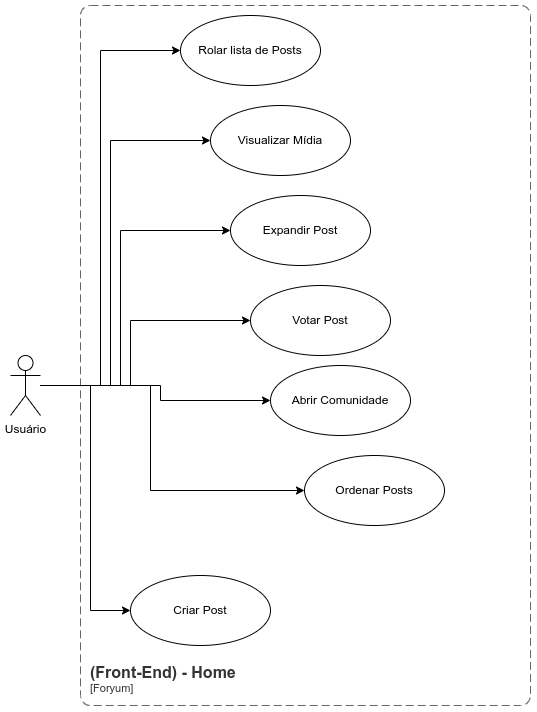
\includegraphics[width=0.9\textwidth]{diagrams/home_diagram.png}
        \caption{Diagrama de casos de uso da tela \textit{home}}\label{fig:home_diagram}
    \end{minipage}
\end{figure}

Junto com os casos de uso, foram definidos as propiedades das entidades do sistema
a partir da criação de um diagrama de classe, o diagrama resultante é exibido
na Figura~\ref{fig:classes_diagram}.

\begin{figure}[h]
    \centering
    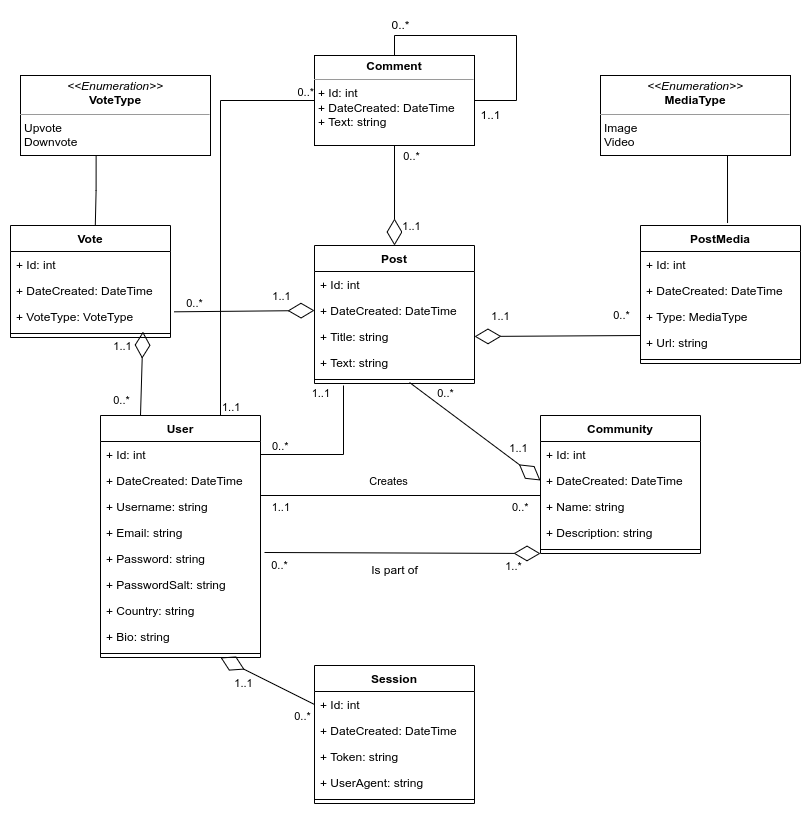
\includegraphics[width=0.8\textwidth]{diagrams/classes_diagram.png}
    \caption{Diagrama de classes do sistema}\label{fig:classes_diagram}
\end{figure}

\subsection{Ambiente de Desenvolvimento}

A ferramenta de desenvolvimento escolhida para implementação
das aplicações foi o \textit{Visual Studio Code} em conjunto com extensões disponíveis
no seu repositório para facilitar seu uso com as tecnologias escolhidas para o projeto. Além
da própria ferramenta de desenvolvimento, foi necessário a instalação dos SDKs
(Kit de Desenvolvimento) das tecnologias que foram utitlizadas. Foram eles o \textit{dotnet} para a implementação do \textit{WebService},
em conjunto com o \textit{Node.js} e \textit{Vue CLI} para implementação do cliente \textit{web}.

Foi utilizado, como auxílio para o desenvolvimento do \textit{WebService} que é uma API REST, o
\textit{software} \textit{Insomnia REST Client} para realização de testes.

Para a criação do banco de dados \textit{MySQL} foi utilizado a ferramenta \textit{Docker} para
seu gerenciamento via contâiner, e para acesso e manipulação desse \textit{MySQL} foi utilizado o software \textit{Dbeaver}.
Além dessas ferramentas, foi utlilizado o site \textit{mockaroo} que oferece \textit{scripts} para preenchimento
de banco de dados com informações de testes. Facilitando o processo de desenvolvimento.

\subsection{Implementação}

Como mencionado anteriormente, foi utilizado um quadro \textit{Kanban} para gerenciamento
de tarefas e a implementação dos sistemas foi realizada com base no quadro \textit{Kanban}.
Para a implementação de algumas dessas houve a necessidade de aprendizagem para sua implementação.

Alguns dos aspectos técnicos que foram implementados no sistema são mostrados nas
Seções~\ref{Autenticacao} e~\ref{Armazenamento}.

\subsubsection{Autenticação}\label{Autenticacao}

O sistema impede que qualquer operação seja realizada se o usuário não estiver autenticado, salvo
apenas a funcionalidade de cadastro. Para isso, existe um mecanismo de autenticação que foi implementado no
sistema `Foryum', esse mecanismo é chamado de \textit{Bearer Token} e ele funciona de acordo com a Figura~\ref{fig:token}.

\begin{figure}[h]
    \centering
    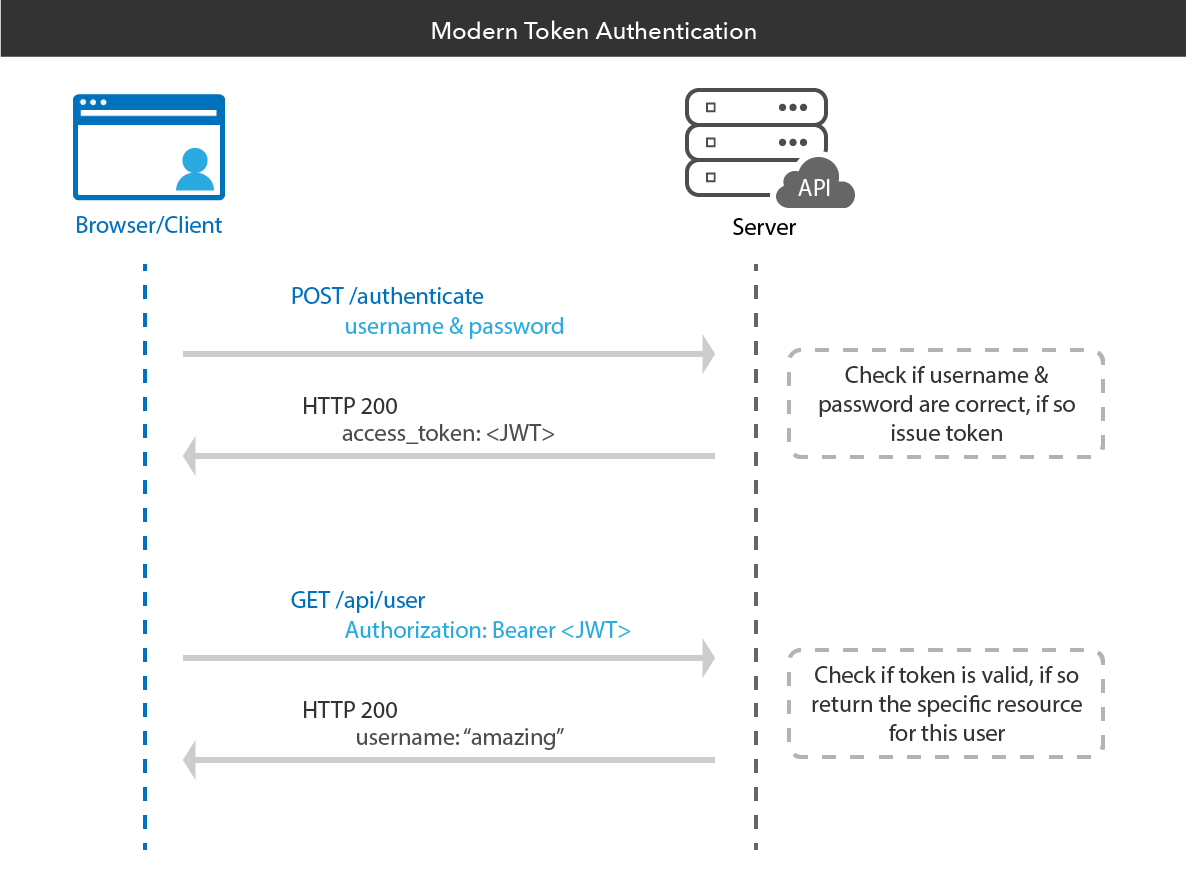
\includegraphics[width=0.5\textwidth]{security/token-authentication.png}
    \caption{Autenticação por Bearer Token}\label{fig:token}
\end{figure}

Nesse mecanismo, o cliente após efetuar o Login no sistema, recebe um \textit{token}. A partir desse momento
o cliente passa a enviar esse token em todas as requisições subsequentes, dessa maneira o servidor
sabe quem o cliente é e que está autenticado.

\subsubsection{Armazenamento de Senhas}\label{Armazenamento}

Outra questão relacionada a segurança é o armazenamento de senhas em banco de dados, nunca
se deve armazenar senhas em texto plano. No sistema foi implementado um processo de armazenamento
de senhas que é chamado de \textit{Password Hash Salting}.

O funcionamento desse processo é visualizado na Figura~\ref{fig:salt}.

\begin{figure}[h]
    \centering
    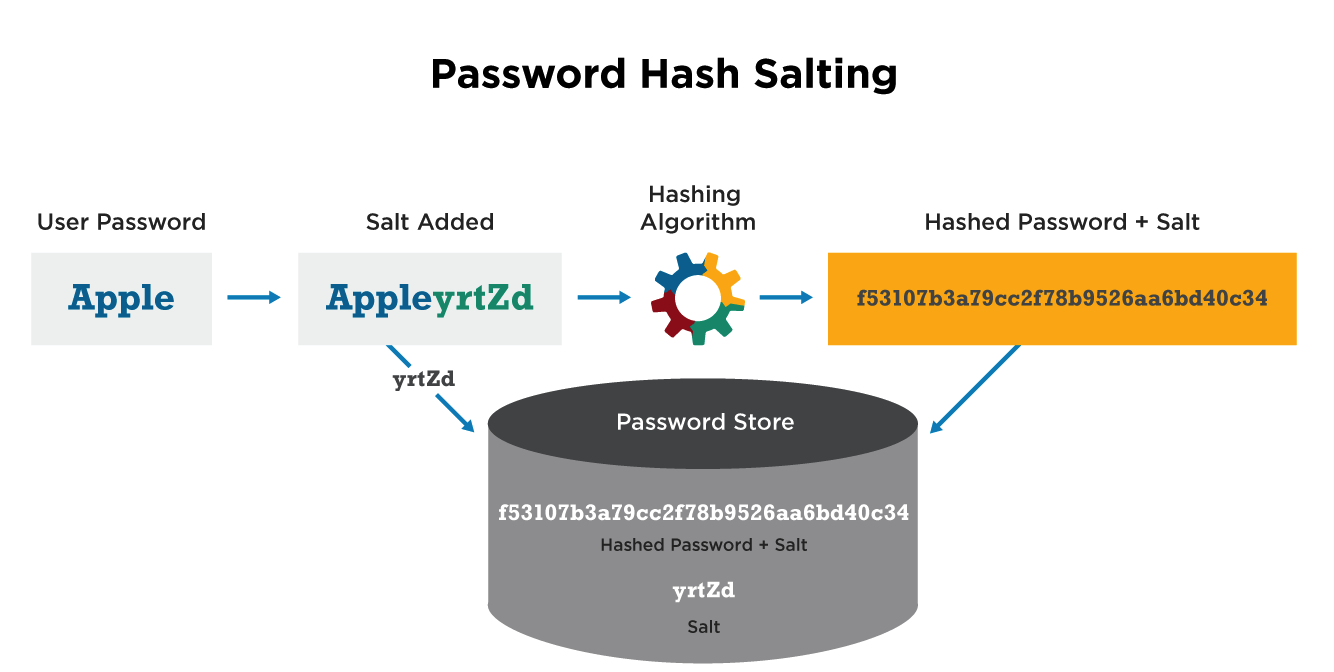
\includegraphics[width=0.5\textwidth]{security/password-salt.png}
    \caption{Processo de \textit{Salting} de uma senha}\label{fig:salt}
\end{figure}

Nesse processo, é concatenado uma string gerada aleatoriamente em uma senha, a partir do resultado
dessa concatenação, um \textit{Hash} é gerado e esse valor é armazenado no banco junto com o \textit{Salt}.

Esse processo, para maior eficiência deve possuir \textit{Salts} diferentes para cada usuário em um banco de dados.
Armazenar senhas dessa maneira evita ataques conhecidos como \textit{Rainbow Table Attack}.

\subsection{Documentação}

Após a finalização da implementação das aplicações, foi construída uma documentação
dos \textit{softwares}, essa documentação foi feita na plataforma \textit{GitHub} na funcionalidade
de \textit{Wiki}. Foi criada uma \textit{Wiki} em cada repositório da aplicação, uma para a aplicação em \textit{Vue,js}
e outra para a API em \textit{.NET}

\section{Resultados}\label{Resultados}

As duas aplicações foram implementadas junto com todas as funcionalidades propostas.
As Figuras~\ref{fig:welcome} e~\ref{fig:home} mostram o resultado da aplicação \textit{Web},
mostrando a tela de Bem-Vindo e a tela Home, respectivamente.

\begin{figure}[h]
    \centering
    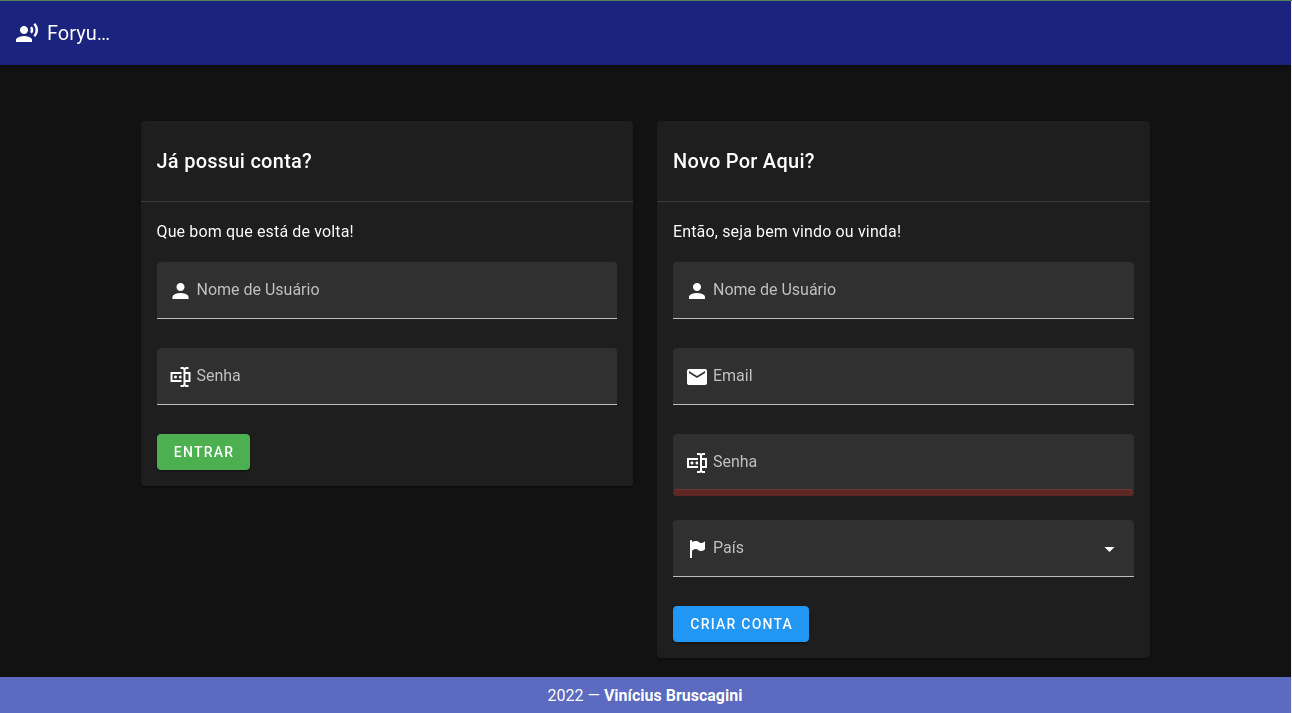
\includegraphics[width=0.8\textwidth]{prints/welcome.png}
    \caption{Tela de bem-vindo}\label{fig:welcome}
\end{figure}

\begin{figure}[h]
    \centering
    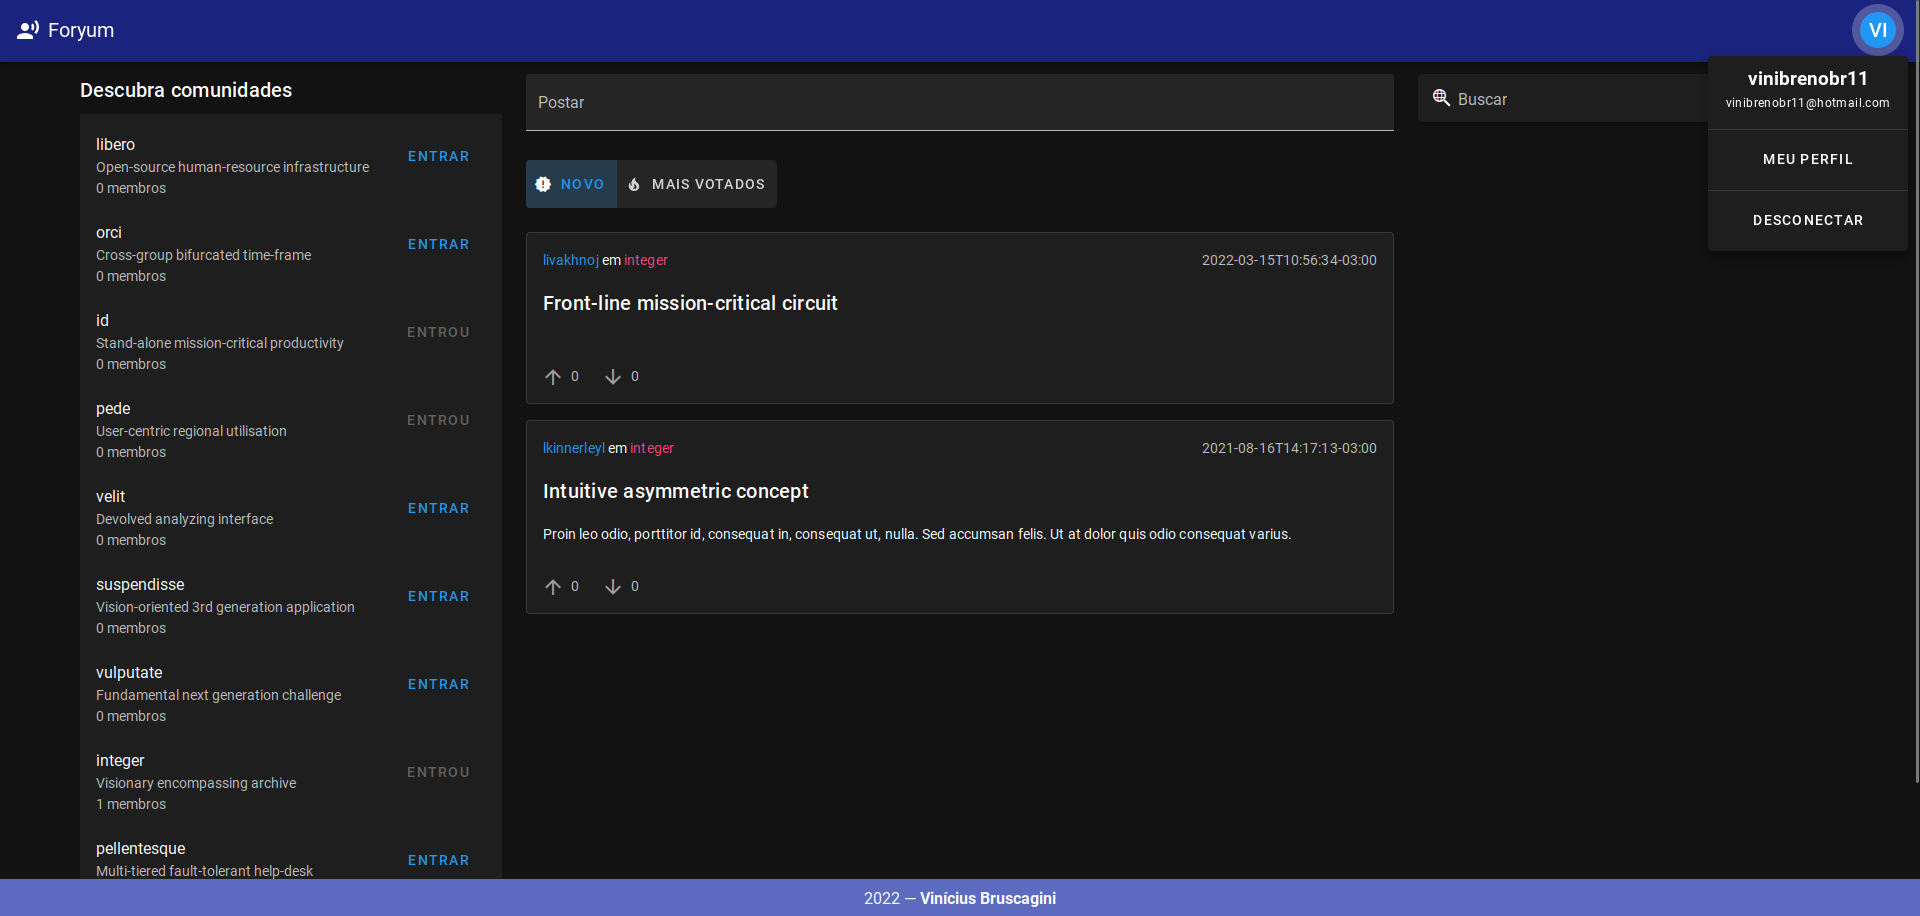
\includegraphics[width=0.8\textwidth]{prints/home.png}
    \caption{Tela \textit{home}}\label{fig:home}
\end{figure}

O Desenvolvimento da API em \textit{.NET} foi finalizadada e todas as funcionalidades
usadas pela aplicação \textit{Web} foram implementadas com restrições de acesso e esquemas de
segurança usando o \textit{Bearer Token}.

Além do desenvolvimento, foi criada a documentação técnica dessas aplicações que estão
na \textit{Wiki} dos repositórios \textit{Git}. Além dos arquivos \textit{README} que mostram
uma introdução das aplicações na tela do repositório.

Os repositórios estão localizados nos \textit{links} especificados a seguir:
\begin{itemize}
  \item https://github.com/V11-0/ForyumServer (WebService);
  \item https://github.com/V11-0/ForyumWeb (Aplicação Web).
\end{itemize}

\section{Conclusão}\label{Conclusao}

O artigo mostrou a dificuldade do ensino em relação as novas tecnologias no desenvolvimento de \textit{software}
e propôs a criação de um sistema com uma documentação técnica para ajudar estudandes em relação a alguns dos
conceitos e tecnologias usadas no desenvolvimento de \textit{software}, além de prover uma abordagem prática
sobre o assunto. Foram implementados duas aplicações sendo um \textit{WebService} com tecnologias \textit{.NET} e
uma aplicação \textit{web} com o \textit{framework Vue}. O código fonte e a documentação técnica dessas duas aplicações
estão disponíveis \textit{online} na plataforma \textit{GitHub}.

Para criação desse trabalho, foram articulados conhecimentos obtidos atráves das disciplinas listadas abaixo, que
são disciplinas que fazem parte da carga horária do curso de Análise e Desenvolvimento de Sistemas do Instituto
Federal de São Paulo - Campus Hortolândia:

\begin{itemize}
  \item Engenharia de Software;
  \item Inglês Técnico Avançado;
  \item Banco de Dados II;
  \item Interação Humano-Computador;
  \item Programação Orientada a Objetos;
  \item Arquitetura de Software;
  \item Qualidade de Software;
  \item Segurança da Informação;
  \item Desenvolvimento de Sistemas Web.
\end{itemize}

Como trabalhos futuros, uma pesquisa de opinião poderia ser feita para estudantes de TI em relação ao material
disponibilizado por este trabalho. Além da documentação, outros conceitos que não foram abrangidos nesse trabalho poderiam
ser explorados como questão de \textit{Pipelines} para realização de entrega contínua (\textit{CI/CD}).
Outra recomendação poderia ser o aprimoramento e criação de novos recursos para o \textit{software} criado nesse trabalho, tais recursos
poderiam ser o \textit{upload} de mídias e gerenciamento de sessões, por exemplo.

\bibliographystyle{sbc}
\bibliography{bibliografia}

\end{document}
